\documentclass[10pt,aspectratio=169]{beamer}
%\documentclass[12pt,aspectratio=169]{beamer}

%\mode<presentation>

\usepackage{graphicx}
\usepackage{breqn}
\usepackage{bm}
\usepackage{color}
\usepackage{tabularx}

\usepackage{listings}
\lstset{language=C++}

\usepackage{mathtools}
\DeclarePairedDelimiter\ceil{\lceil}{\rceil}
\DeclarePairedDelimiter\floor{\lfloor}{\rfloor}



\definecolor{radeonruby}{rgb}{0.87, 0, 0.19}


\usepackage{listings}



%\usepackage[utf8]{inputenc}
\definecolor{bluekeywords}{rgb}{0.63, 0.79, 0.95}
\definecolor{greencomments}{rgb}{0,0.5,0}
\definecolor{redstrings}{rgb}{0.64,0.08,0.08}
\definecolor{xmlcomments}{rgb}{0.5,0.5,0.5}
\definecolor{types}{rgb}{0.17,0.57,0.68}
\lstset{language=C++,
captionpos=b,
%numbers=left,
%numberstyle=\tiny,
frame=single,
showspaces=false,
showtabs=false,
breaklines=true,
showstringspaces=false,
breakatwhitespace=true,
escapeinside={(*@}{@*)},
commentstyle=\color{greencomments},
morekeywords={partial, var, value, get, set},
keywordstyle=\color{bluekeywords},
stringstyle=\color{redstrings},
basicstyle=\ttfamily\small,
}

\usepackage[yyyymmdd]{datetime}
\renewcommand{\dateseparator}{--}

%\usepackage[inline]{asymptote}
\usepackage{asymptote}
\def\asylatexdir{}
\def\asydir{}

\renewcommand{\thefootnote}{\fnsymbol{footnote}}

\def\clap#1{\hbox to 0pt{\hss#1\hss}}
\def\mathllap{\mathpalette\mathllapinternal}
\def\mathrlap{\mathpalette\mathrlapinternal}
\def\mathclap{\mathpalette\mathclapinternal}
\def\mathllapinternal#1#2{\llap{$\mathsurround=0pt#1{#2}$}}
\def\mathrlapinternal#1#2{\rlap{$\mathsurround=0pt#1{#2}$}}
\def\mathclapinternal#1#2{\clap{$\mathsurround=0pt#1{#2}$}}

\def\p{\pause}

\def\({\left(}
\def\){\right)}
\def\[{\left[}
\def\]{\right]}

\def\no#1{\nobreak{#1}} % stop equation breaking in dmath

\begin{asydef}
  // Global Asymptote definitions can be put here.
  import three;
  usepackage("bm");
  texpreamble("\def\V#1{\bm{#1}}");
  // One can globally override the default toolbar settings here:
  // settings.toolbar=true;
\end{asydef}

%\useinnertheme{rectangles} %specifies itemize points to be rectangles
\useoutertheme{default}

\definecolor{darkgreen}{RGB}{0, 100, 0}
\definecolor{brightpurple}{RGB}{160,32,240}

% fg specifies foreground color
% bg specifies background color
% the notation color!x!white mixes the color with 1-x amount of white
%\setbeamercolor{frametitle}{fg=darkgreen!90!black, bg=darkgreen!10!white}
\setbeamercolor{normal text}{fg=white,bg=black}
% defines color of structure elements, e.g., color of text in the
% outline, block titles many more definitions possible. Each element
% predefined by the theme can be overwritten individually

\setbeamerfont{author}{size=\small,series=\bfseries,parent=structure}

\setbeamercolor{background canvas}{bg=white}
%% \usebackgroundtemplate
%% {
%%   
\includegraphics[width=\paperwidth,height=\paperheight]{gpu_background_black.png}
%% }
\pgfdeclareimage[width=\paperwidth]{mybackground}{../talks/siampp20/gpu_background_black.png}
\setbeamertemplate{title page}{
  \begin{picture}(0,0)
    \put(-30,-163){%
      \pgfuseimage{mybackground}
    }
    \put(0,-150){%
      \begin{minipage}[b][45mm][t]{226mm}
        \usebeamerfont{title}{\inserttitle\par}
        \ifx\insertsubtitle\@empty%
        \else%
        {\vskip0.25em%
        \usebeamerfont{subtitle}\usebeamercolor[fg]{subtitle}\insertsubtitle\par}%
        \fi%
        \vskip1cm%              
        \usebeamerfont{author}{\insertauthor\par}
        \usebeamerfont{date}\url{malcolm.roberts@amd.com}\par
        \usebeamerfont{date}\insertdate
      \end{minipage}
    }
  \end{picture}
}

%------------------------------------------------------------------------
%------------------------------------------------------------------------



\def\thetitle{rocFFT}
\def\thesubtitle{Statistical Methods for Performance Analysis}
\def\theauthor{rocFFT group}
\def\theauthorinstitute{AMD}

\def\presdate{2023-01-11}

\hypersetup{
  pdftitle=\thetitle{} \thesubtitle{},
  pdfauthor=\theauthor{}
}

\title{\thetitle{}}
\subtitle{\thesubtitle{}}
\author{\theauthor{}}
\institute{\theauthorinstitute}
\date{\presdate}

\setbeamertemplate{frametitle}[default][center]
%\setbeamertemplate{footline}[frame number]
\setbeamertemplate{navigation symbols}{} 

\begin{document}

\setbeamertemplate{headline}{}
%\setbeamertemplate{footline}{}

{
  \setbeamercolor{background canvas}{bg=black}
  \setbeamercolor{normal text}{fg=white,bg=black}
  \setbeamercolor{frametitle}{fg=white}
  \setbeamercolor{title}{fg=white}
  \setbeamercolor{alerted text}{fg=white}
  \setbeamercolor{structure}{fg=white}
  \usebeamercolor[fg]{normal text}
  \begin{frame}
    \titlepage
  \end{frame}
}


\setbeamercolor{normal text}{fg=black,bg=white}
\usebeamercolor[fg]{normal text}

\newcolumntype{R}{>{\raggedleft\arraybackslash}X}
\setbeamertemplate{footline}{
   \leavevmode%
   \hbox{%
     \begin{beamercolorbox}[wd=\paperwidth,ht=1ex,dp=1.125ex]{author in head/foot}%
  \begin{tabularx}{\paperwidth}{lR}
    \hfill\insertframenumber/\inserttotalframenumber\hfill\phantom{.}%
    & %
    
\includegraphics[width=0.05\textwidth]{../talks/siampp20/footerlogo}%
    \\%
  \end{tabularx}%
  \end{beamercolorbox}%
  }%
}




\begin{frame}
  \frametitle{Motivation}

  
  \begin{columns}[T] % align columns
    \begin{column}{.48\textwidth}

      \begin{center}
        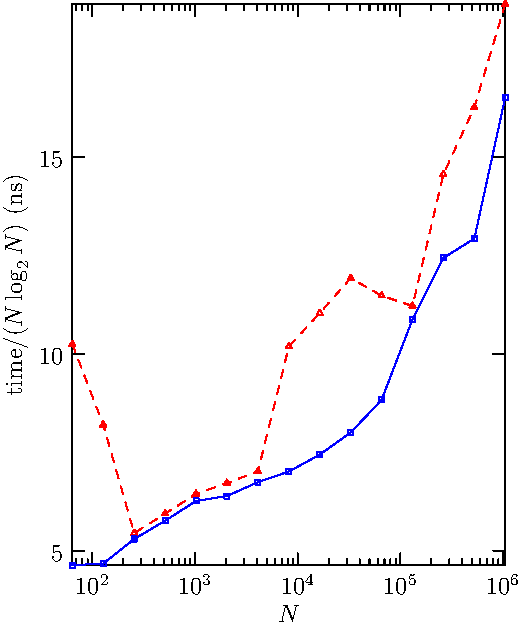
\includegraphics[width=0.9\textwidth]{pdf/atlas_cconv}
      \end{center}

      
    \end{column}%
    \hfill%
    \begin{column}{.48\textwidth}

      \vspace{1cm}
      
      Benchmarking algorithms allows us to
      \begin{itemize}
      \item Optimize libraries
      \item Detect regressions
      \item Tune implementations
      \end{itemize}

      \medskip
      The graph shows a comparison:
      \begin{itemize}
      \item from a single CPU core
      \item at low load, headless
      \item Lots of samples (mean shown)
      \item Blue implementation is clearly superior
      \end{itemize}

      \bigskip
      
      Problem: it's just the same thing run twice.
      
    \end{column}%
  \end{columns}

  
\end{frame}

\begin{frame}
    \frametitle{Problem}
    
    Common strategies:
    \begin{itemize}
    \item Run 10 times, take the minimum
      \begin{itemize}
      \item Idea: show the ``power'' of the device.
      \item \dots{} but we have no confidence that we got the minimum.
      \end{itemize}
    \item Plot the data
      \begin{itemize}
      \item Idea: if the lines are on top of each other, call it a wash.
      \item \dots{} that's a lot of graphs to look at.
      \item \dots{} this doesn't automate well.
      \end{itemize}
    \item Cut-off based on effect size
      \begin{itemize}
      \item Idea: if the difference is $<5\%$, call it a wash.
      \item \dots{} what if we have two regressions of $3\%$?
      \end{itemize}
    \end{itemize}
    
    \medskip
    \begin{center}
      How can we build confidence in our performance tests?
    \end{center}
    
\end{frame}

\begin{frame}
  \frametitle{Problem}


  \bigskip
  
  Two relevant CppCon talks (2015):
  \begin{itemize}
  \item \href{https://www.youtube.com/watch?v=zWxSZcpeS8Q}{Bryce Adelstein-Lelbach “Benchmarking C++ Code"}
    \begin{itemize}
    \item FIXME: main points
    \item Macro benchmarks
    \end{itemize}
  \item \href{https://www.youtube.com/watch?v=nXaxk27zwlk}{Chandler Carruth ``Tuning C++: Benchmarks, and CPUs, and Compilers! Oh My!''}
    \begin{itemize}
    \item FIXME: main points
    \item Micro benchmarks
    \item google/benchmark
    \item Underlying code gives the mean and standard deviation
    \end{itemize}
  \end{itemize}
  
\end{frame}


\begin{frame}
  \frametitle{Problem}
  \begin{center}
    Things seem to be a bit better on the GPU:
  \end{center}
  \begin{center}
    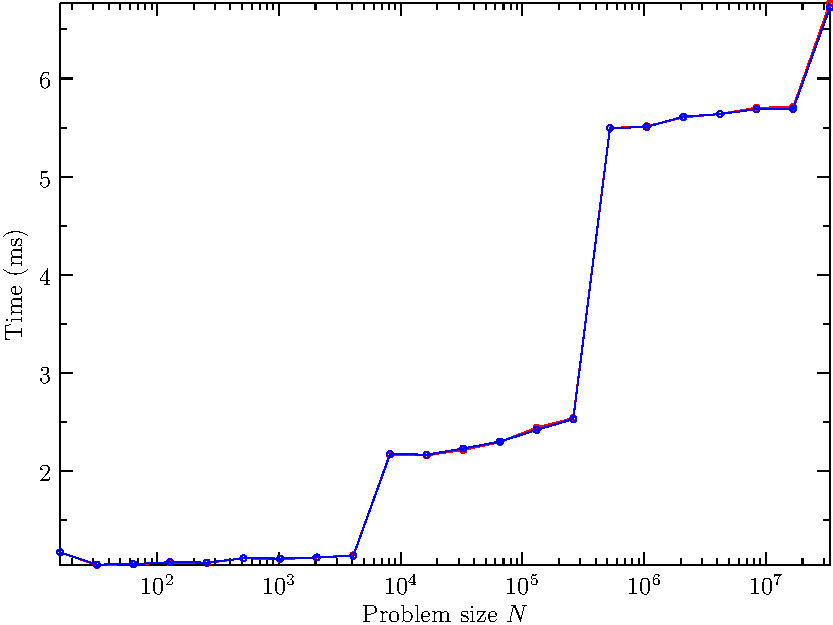
\includegraphics[width=0.7\textwidth]{pdf/footprint2exp25_1D_double_forward_complex_out-of-place}
  \end{center}
  % measure=mean
  
  
%    asy -f pdf /home/mal/repo/rocfft/scripts/perf/datagraphs.asy -u 'filenames="/home/mal/sync/amd/ntrial/ixt-hq-107/sep/foot/8/a/footprint2exp25_1D_double_forward_complex_out-of-place.mdat,/home/mal/sync/amd/ntrial/ixt-hq-107/sep/foot/8/aa/footprint2exp25_1D_double_forward_complex_out-of-place.mdat";dobars=false;dolegend=false;Ncut=1000' -o footprint2exp25_1D_double_forward_complex_out-of-place_cut_1000.pdf

  
\end{frame}
  

\begin{frame}
  \frametitle{Problem}
  \begin{center}
    Though it's a little less clear if we zoom in:
  \end{center}
  \begin{center}
    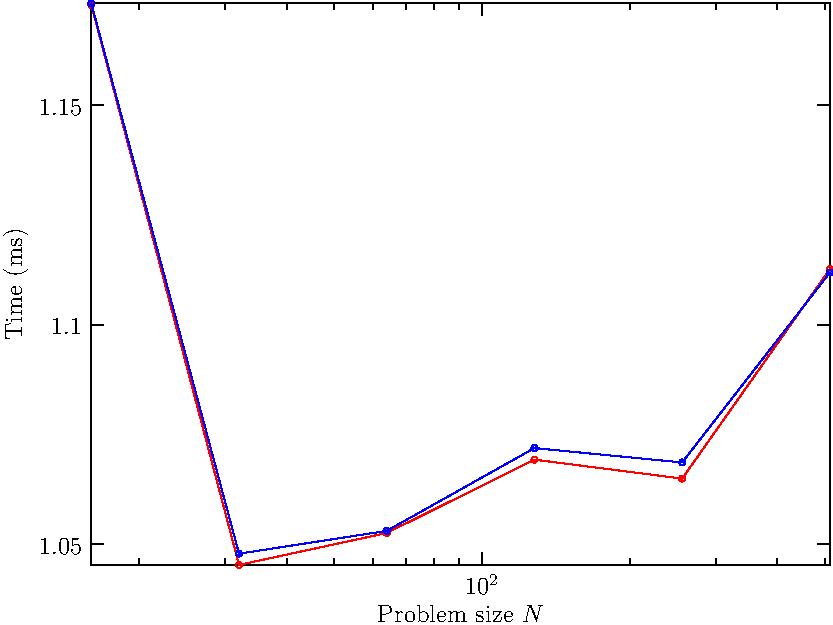
\includegraphics[width=0.7\textwidth]{pdf/footprint2exp25_1D_double_forward_complex_out-of-place_cut_1000}
  \end{center}
  % measure=mean
  


%    asy -f pdf /home/mal/repo/rocfft/scripts/perf/datagraphs.asy -u 'filenames="/home/mal/sync/amd/ntrial/ixt-hq-107/sep/foot/8/a/footprint2exp25_1D_double_forward_complex_out-of-place.mdat,/home/mal/sync/amd/ntrial/ixt-hq-107/sep/foot/8/aa/footprint2exp25_1D_double_forward_complex_out-of-place.mdat";dobars=false;dolegend=false;Ncut=1000' -o footprint2exp25_1D_double_forward_complex_out-of-place_cut_1000.pdf

  
\end{frame}

\begin{frame}
  \frametitle{Problem}
  \begin{center}
    Let's look at the data more closely!
  \end{center}
  \begin{center}
    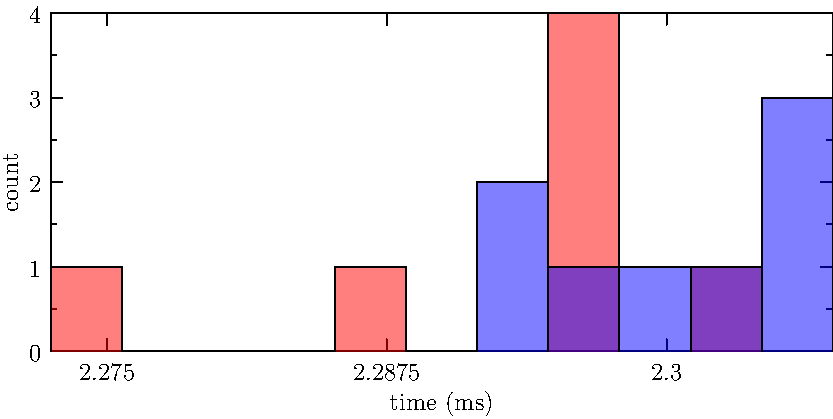
\includegraphics[width=0.7\textwidth]{pdf/histogram_ixt-hq-107_sep_8_64k_b512.pdf}
  \end{center}
% asy -f pdf -u'filelist="/home/mal/sync/amd/ntrial/ixt-hq-107/sep/foot/8/a/footprint2exp25_1D_double_forward_complex_out-of-place.dat,/home/mal/sync/amd/ntrial/ixt-hq-107/sep/foot/8/aa/footprint2exp25_1D_double_forward_complex_out-of-place.dat";token="complex_forward_len_65536_double_op_batch_512_istride_1_CI_ostride_1_CI_idist_65536_odist_65536_ioffset_0_0_ooffset_0_0"' histogram.asy -o histogram_ixt-hq-107_sep_8_64k_b512.pdf


  \begin{center}
    Ok, maybe not.  Do we need more data?
  \end{center}
  
\end{frame}

\begin{frame}
  \frametitle{Problem}
  \begin{center}
    Let's look at the data more closely!
  \end{center}
  \begin{center}
    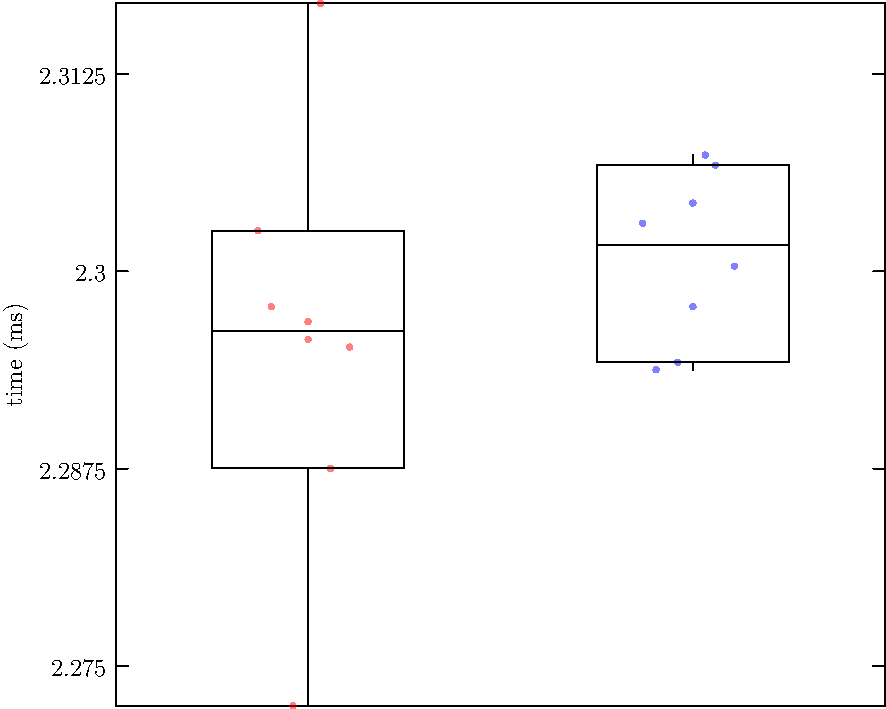
\includegraphics[width=0.5\textwidth]{pdf/whisker_ixt-hq-107_sep_8_64k_b512.pdf}
  \end{center}
%asy -f pdf -u'filelist="/home/mal/sync/amd/ntrial/ixt-hq-107/sep/foot/8/a/footprint2exp25_1D_double_forward_complex_out-of-place.dat,/home/mal/sync/amd/ntrial/ixt-hq-107/sep/foot/8/aa/footprint2exp25_1D_double_forward_complex_out-of-place.dat";token="complex_forward_len_65536_double_op_batch_512_istride_1_CI_ostride_1_CI_idist_65536_odist_65536_ioffset_0_0_ooffset_0_0"' plot.asy -o whisker_ixt-hq-107_sep_8_64k_b512.pdf

  \begin{center}
    Still need more data.
  \end{center}
  
\end{frame}

\begin{frame}
  \frametitle{Problem}
  \begin{center}
    More data!  ($N=8192$ - you're patient, right?)
  \end{center}
  \begin{center}
    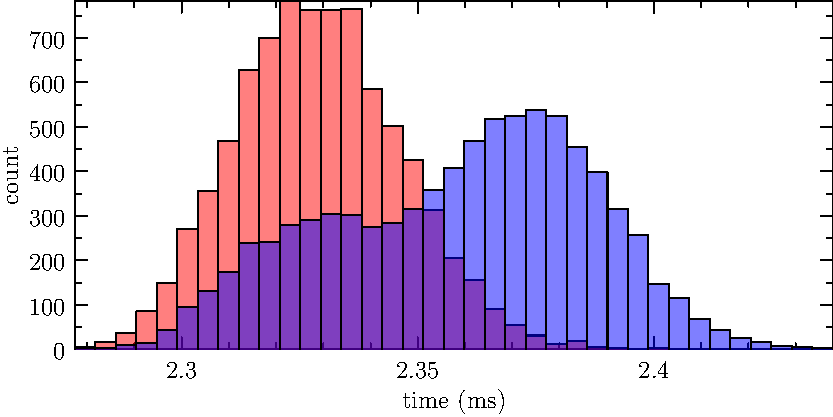
\includegraphics[width=0.7\textwidth]{pdf/histogram_ixt-hq-107_sep_8192_64k_b512.pdf}
  \end{center}
  % measure=mean
% asy -f pdf -u'filelist="/home/mal/sync/amd/ntrial/ixt-hq-107/sep/foot/8192/a/footprint2exp25_1D_double_forward_complex_out-of-place.dat,/home/mal/sync/amd/ntrial/ixt-hq-107/sep/foot/8192/aa/footprint2exp25_1D_double_forward_complex_out-of-place.dat";token="complex_forward_len_65536_double_op_batch_512_istride_1_CI_ostride_1_CI_idist_65536_odist_65536_ioffset_0_0_ooffset_0_0"' histogram.asy -o histogram_ixt-hq-107_sep_8192_64k_b512.pdf

\end{frame}

\begin{frame}
  \frametitle{Problem}
  \begin{center}
    Let's look at the data more closely!
  \end{center}
  \begin{center}
    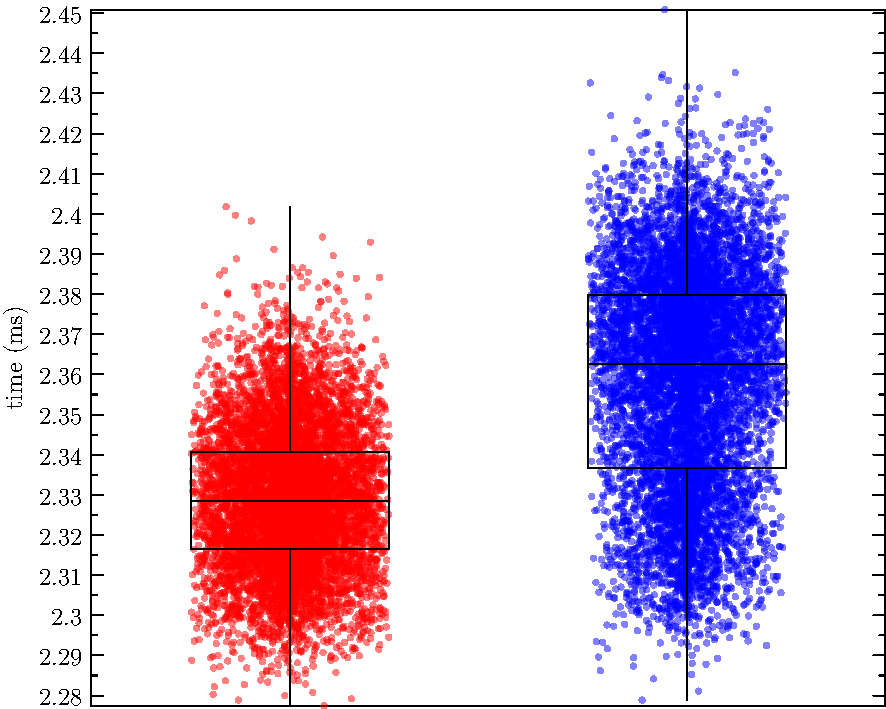
\includegraphics[width=0.5\textwidth]{pdf/whisker_ixt-hq-107_sep_8192_64k_b512.pdf}
  \end{center}
%asy -f pdf -u'filelist="/home/mal/sync/amd/ntrial/ixt-hq-107/sep/foot/8192/a/footprint2exp25_1D_double_forward_complex_out-of-place.dat,/home/mal/sync/amd/ntrial/ixt-hq-107/sep/foot/8192/aa/footprint2exp25_1D_double_forward_complex_out-of-place.dat";token="complex_forward_len_65536_double_op_batch_512_istride_1_CI_ostride_1_CI_idist_65536_odist_65536_ioffset_0_0_ooffset_0_0"' plot.asy -o whisker_ixt-hq-107_sep_8192_64k_b512.pdf

  \begin{center}
    More data did not help!  \texttt{\textbackslash{}tex\_command\_for\_sad\_face}
  \end{center}
  
\end{frame}


\begin{frame}
  \frametitle{More problems: speedup is even noisier!}

  \begin{center}
    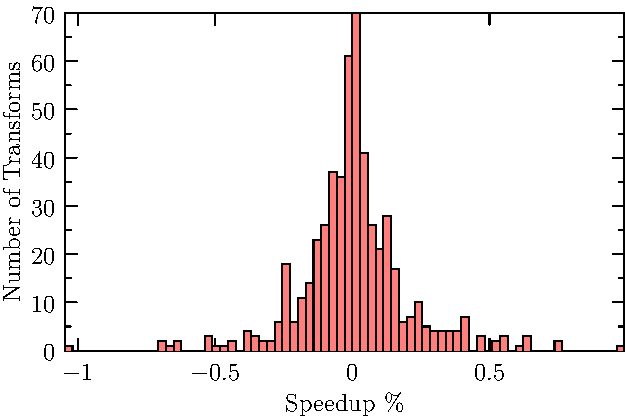
\includegraphics[width=0.5\textwidth]{pdf/histogram_ixt-hq-107_sep_8_speedup.pdf}
  \end{center}

  Histogram of speedups over a suite of tests
  \begin{itemize}
  \item 534 different tests
  \item 8 samples per tests
  \item This is what a null result looks like.
  \end{itemize}

\end{frame}


\begin{frame}
  \frametitle{More problems: speedup is even noisier!}

  \begin{center}
    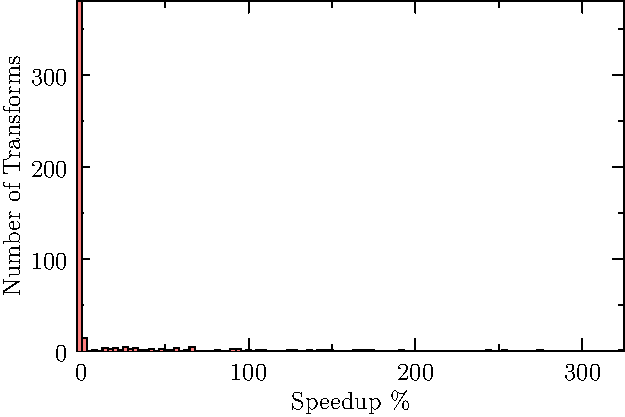
\includegraphics[width=0.5\textwidth]{pdf/histogram_ixt-hq-107_sep_8192_speedup.pdf}
  \end{center}

% nice -n 19 ./rocfft-perf pdf ~/sync/amd/ntrial/ixt-hq-107/sep/foot/8192/doc ~/sync/amd/ntrial/ixt-hq-107/sep/foot/8192/a ~/sync/amd/ntrial/ixt-hq-107/sep/foot/8192/aa --measure mean --significance 2
  
  Histogram of speedups over a suite of tests
  \begin{itemize}
  \item 534 different tests
  \item 8192 samples per tests
  \item This null result looks even worse!
  \end{itemize}

\end{frame}

\begin{frame}
  \frametitle{Proposed solution}
  \begin{center}
    Always use a \textcolor{radeonruby}{red} pen to colour your data.
  \end{center}

  \medskip
  
  \begin{itemize}
  \item \textcolor{radeonruby}{Red}-labelled data has lower execution time.
    \medskip
  \item \textcolor{radeonruby}{Robust} over three orders of magnitude
    of sample sizes.
    \medskip
  \item Appropriate \textcolor{radeonruby}{AMD} branding.
    \medskip
  \item \texttt{\textbackslash{}definecolor\{\textcolor{radeonruby}{radeonruby}\}\{rgb\}\{0.87, 0, 0.19\}}
  \end{itemize}

  % NB: CPU data was on an intel machine, so the red-labelling
  % solution doesn't apply.
  
\end{frame}


\begin{frame}
    \frametitle{Actual proposed solution}

    Problem:
    \begin{itemize}
    \item Performance tests are suprisingly noisy.
    \item The noise isn't the same over tests
    \end{itemize}
        
    \bigskip

    Solution:
    \begin{itemize}
    \item Choose an experimental design that eliminates bias.
    \item Use statistical tests to handle noise.
    \end{itemize}

\end{frame}

\begin{frame}
  \frametitle{Experimental design}

  
    \begin{itemize}    
    \item Noise (aka jitter) is a fact of life.
      \medskip
    \item We can't do statistical tests if the noise isn't identically
      distributed.
      \medskip
    \item Some runs get more noise - why?  What can we do?
    \end{itemize}
  
\end{frame}

\begin{frame}
    \frametitle{Separated Design}

    Our experimental setup:
    \begin{itemize}
    \item Intitialize with rocRand/hipRand
    \item Run on the same node
    \item Separate processes, one right after the other.
    \end{itemize}

    \bigskip

    \begin{center}
      ``Separated'' experimental design:\\
      \medskip
      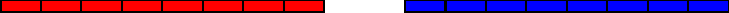
\includegraphics[]{asy/sep.pdf}
    \end{center}
    \bigskip
    
    Maybe some random environmental thing caused an issue - try in the
    same process!
    
\end{frame}

\begin{frame}
    \frametitle{Separated design}

    % asy -f pdf -u'filelist="/home/mal/sync/amd/ntrial/ixt-hq-107/sep/foot/8192/a/footprint2exp28_1D_double_forward_complex_out-of-place.dat,/home/mal/sync/amd/ntrial/ixt-hq-107/sep/foot/8192/aa/footprint2exp28_1D_double_forward_complex_out-of-place.dat";token="complex_forward_len_16384_double_op_batch_16384_istride_1_CI_ostride_1_CI_idist_16384_odist_16384_ioffset_0_0_ooffset_0_0"' histogram.asy  -o  histogram_ixt-hq-107_sep_8192_16k_b16k.pdf
    
    \begin{center}
      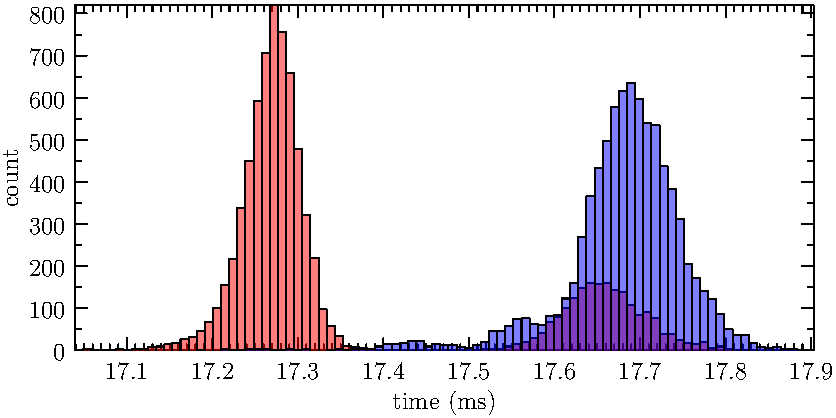
\includegraphics[width=0.8\textwidth]{pdf/histogram_ixt-hq-107_sep_8192_16k_b16k.pdf}
    \end{center}

    \begin{center}
      Our data looks terrible!
      \medskip
      \begin{itemize}
      \item Hard-pressed to believe that this is the same code.
      \item Statistics will not save us from bad data.
      \end{itemize}
    \end{center}

\end{frame}


\begin{frame}
    \frametitle{Sequential Design}

    \begin{itemize}    
    \item Load two versions of the implementation into the same executable
      \begin{itemize}
      \item How?  Abuse \texttt{dload}!
      \item Libraries must not depend on other shared libraries: \texttt{-DSINGLELIB} in rocFFT.
      \end{itemize}
    \item We can now guarantee that the environments are identical.
    \end{itemize}

    \bigskip
    
    New experimental setup:
    \begin{center}
      ``Sequential'' experimental design:\\
      \medskip
      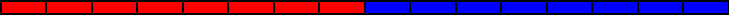
\includegraphics[]{asy/seq.pdf}
    \end{center}

    
    
\end{frame}


\begin{frame}
    \frametitle{Sequential experimental design}

    %asy -f pdf -u'filelist="/home/mal/sync/amd/ntrial/ixt-hq-107/seq/foot/8192/a/footprint2exp28_1D_double_forward_complex_out-of-place.dat,/home/mal/sync/amd/ntrial/ixt-hq-107/seq/foot/8192/aa/footprint2exp28_1D_double_forward_complex_out-of-place.dat";token="complex_forward_len_16384_double_op_batch_16384_istride_1_CI_ostride_1_CI_idist_16384_odist_16384_ioffset_0_0_ooffset_0_0"' histogram.asy  -o  histogram_ixt-hq-107_seq_8192_16k_b16k.pdf

    % FIXME: add run details
    
    \begin{center}
      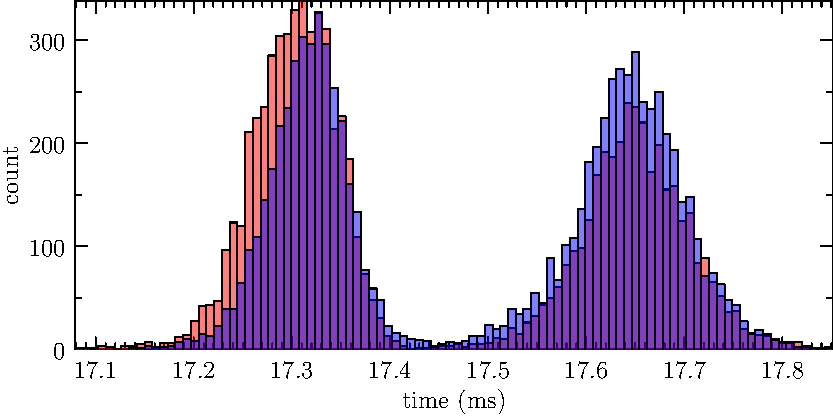
\includegraphics[width=0.8\textwidth]{pdf/histogram_ixt-hq-107_seq_8192_16k_b16k.pdf}
    \end{center}

    \begin{center}
      Better!
      \medskip
      \begin{itemize}
      \item Distributions are closer.
      \item But not that close!
      \end{itemize}
    \end{center}

\end{frame}

\begin{frame}
  \frametitle{Sequential experimental design}

  \begin{center}
    Hypothesis:
  \end{center}

  \bigskip

  The device is intermittently interrupted.

  \bigskip

  This interruption is time-correlated.

  \bigskip
  
  Therefore, the noise is time-correlcated.

  \bigskip

  To decorrelate noise and test case, we must de-correlate test case
  with time.
    
  
\end{frame}

\begin{frame}
    \frametitle{Alternating Design}

    Since we have both cases \texttt{dload}ed into one executable, we can alternate cases.
    \begin{itemize}
    \item Reduces time/test-case correlation.
    \end{itemize}
    
    \begin{center}
      ``Alternating'' experimental design:\\
      \medskip
      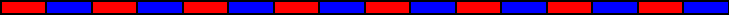
\includegraphics[]{asy/alt.pdf}
    \end{center}
  
    
\end{frame}


\begin{frame}
    \frametitle{Alternating design}

    %asy -f pdf -u'filelist="/home/mal/sync/amd/ntrial/ixt-hq-107/alt/foot/8192/a/footprint2exp28_1D_double_forward_complex_out-of-place.dat,/home/mal/sync/amd/ntrial/ixt-hq-107/alt/foot/8192/aa/footprint2exp28_1D_double_forward_complex_out-of-place.dat";token="complex_forward_len_16384_double_op_batch_16384_istride_1_CI_ostride_1_CI_idist_16384_odist_16384_ioffset_0_0_ooffset_0_0"' histogram.asy  -o  histogram_ixt-hq-107_alt_8192_16k_b16k.pdf

    % FIXME: add run details
    
    \begin{center}
      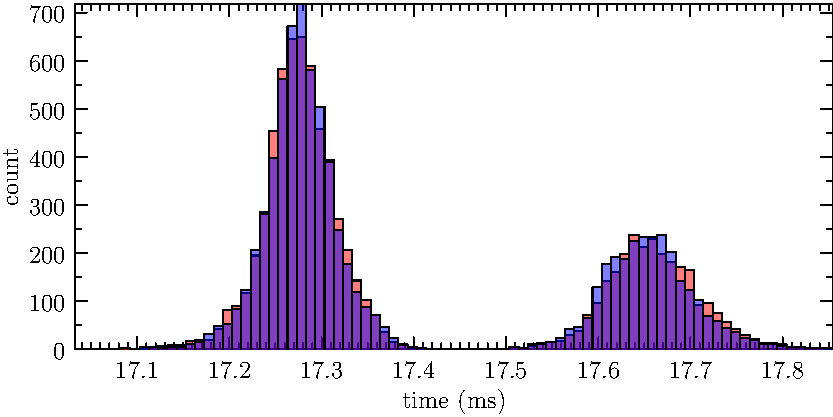
\includegraphics[width=0.8\textwidth]{pdf/histogram_ixt-hq-107_alt_8192_16k_b16k.pdf}
    \end{center}

    \begin{center}
      Better!
      \medskip
      \begin{itemize}
      \item The noise isn't obviously correlated with the test case.
      \end{itemize}
    \end{center}

\end{frame}

\begin{frame}
    \frametitle{Randomized Design}

    Alternating test cases won't eliminate alternating noise.

    \bigskip
    
    \begin{itemize}
    \item If we're alternating we may as well randomize.
    \item Random case choice maximally reduces correlation.
    \item For $N$ samples, either:
      \begin{itemize}
      \item randomly pick a case until we have at lesat $N$ samples per case,
      \item or take the sequential case and shuffle the order.
      \end{itemize}
    \end{itemize}
    
    \begin{center}
      
\includegraphics[]{asy/ran.pdf}
    \end{center}
  
\end{frame}


\begin{frame}
    \frametitle{Randomized experimental design}

    %asy -f pdf -u'filelist="/home/mal/sync/amd/ntrial/ixt-hq-107/alt/foot/8192/a/footprint2exp28_1D_double_forward_complex_out-of-place.dat,/home/mal/sync/amd/ntrial/ixt-hq-107/alt/foot/8192/aa/footprint2exp28_1D_double_forward_complex_out-of-place.dat";token="complex_forward_len_16384_double_op_batch_16384_istride_1_CI_ostride_1_CI_idist_16384_odist_16384_ioffset_0_0_ooffset_0_0"' histogram.asy  -o  histogram_ixt-hq-107_alt_8192_16k_b16k.pdf

    % FIXME: add run details
    
    \begin{center}
      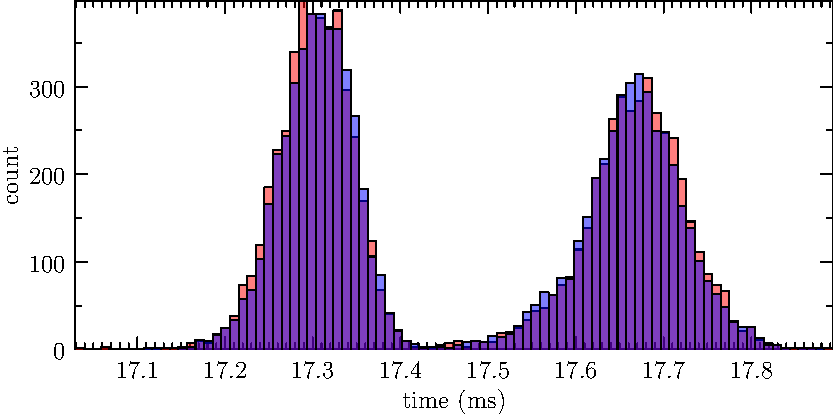
\includegraphics[width=0.8\textwidth]{pdf/histogram_ixt-hq-107_ran_8192_16k_b16k.pdf}
    \end{center}

    \begin{center}
      Much better!
      \medskip
      \begin{itemize}
      \item Noise isn't correlated with case.
      \end{itemize}
    \end{center}

\end{frame}

\begin{frame}
    \frametitle{Characterizing data}

    We can get better data using a randomized experimental design.

    \begin{itemize}
    \item That's some weird-looking data.
    \item How should we evaluate our results?
    \end{itemize}

    \bigskip
    
    What we want:
    \begin{itemize}
    \item A measure of central tendency
    \item Some quantification of uncertainty
    \item A test to tell us when things are different.
    \end{itemize}
    
    
\end{frame}



\begin{frame}
    \frametitle{Measurement of Central Tendency}


    There are two basic measures of central tendency:

    \begin{itemize}
    \item Mean
    \item Median
    \end{itemize}

    Our data can be quite skewed and has outliers \pause{} - the mean
    can be quite unstable in this context.
   
    \begin{center}
      
\includegraphics[width=0.5\textwidth]{img/mean_median_skew_meme.jpg}
    \end{center}
    \pause{}
    
    The median is also stable under monotonic transforms, eg:
    \begin{itemize}
    \item time $\rightarrow$ gflops
    \item time $\rightarrow$ bandwidth
    \end{itemize}
    
\end{frame}

\begin{frame}
    \frametitle{Uncertainty quantification}

    Whichever measure we choose, we need to quantify the uncertainty.

    \bigskip

    The mean is associated with standard deviation
    \begin{itemize}
    \item Assumes a normal distribution
    \item The mean minus the standard deviation is often negative
      \begin{itemize}
      \item Negative values are difficult to plot on log-log plots.
      \end{itemize}
    \end{itemize}

    %\pause
    
    \bigskip
    
    Alternative: bootstrap resampling.
    \begin{itemize}
    \item Given $N$ data points, sample, with replacement $N$ value.
    \item Compute a new statistic (ie mean or median).
    \item Do this a lot (like 2000 times).
    \item The range of the middle $90\%$ values gives the $90\%$
      confidence interval.
    \item Slightly expensive but incredibly robust.
    \end{itemize}
    

\end{frame}


\begin{frame}
    \frametitle{Uncertainty quantification}
    % ./rocfft-perf post ~/sync/amd/ntrial/ixt-hq-107/seq/foot/8192/doc_boot_mean ~/sync/amd/ntrial/ixt-hq-107/seq/foot/8192/a ~/sync/amd/ntrial/ixt-hq-107/seq/foot/8192/aa --measure mean --confidence bootstrap



    %asy -f pdf /home/mal/repo/rocfft/scripts/perf/datagraphs.asy -u 'filenames="/home/mal/sync/amd/ntrial/ixt-hq-107/seq/foot/8192/a/footprint2exp25_1D_double_backward_complex_out-of-place.mdat,/home/mal/sync/amd/ntrial/ixt-hq-107/seq/foot/8192/aa/footprint2exp25_1D_double_backward_complex_out-of-place.mdat";dobars=true;dolegend=false'  -o stdev.pdf

    \begin{center}
      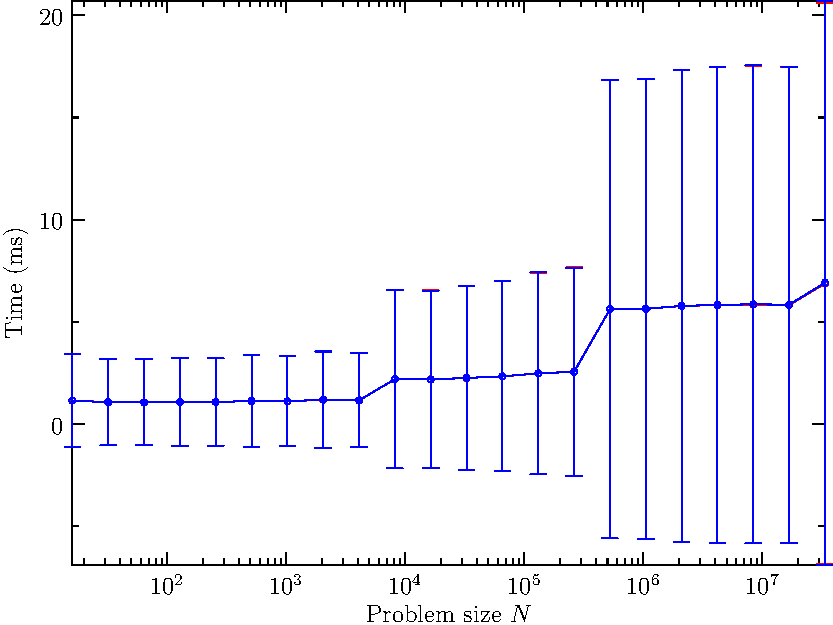
\includegraphics[width=0.5\textwidth]{pdf/stdev.pdf}
    \end{center}

    \begin{center}
      Mean with 95\% interval from standard deviation.
    \end{center}
        
\end{frame}
    
\begin{frame}
    \frametitle{Uncertainty quantification}
    % ./rocfft-perf --verbose  pdf ~/sync/amd/ntrial/ixt-hq-107/seq/foot/8192/doc_mean_boot ~/sync/amd/ntrial/ixt-hq-107/seq/foot/8192/a ~/sync/amd/ntrial/ixt-hq-107/seq/foot/8192/aa --measure mean --confidence bootstrap --significance 2

    %asy -f pdf /home/mal/repo/rocfft/scripts/perf/datagraphs.asy -u 'filenames="/home/mal/sync/amd/ntrial/ixt-hq-107/seq/foot/8192/a/footprint2exp25_1D_double_backward_complex_out-of-place.mdat,/home/mal/sync/amd/ntrial/ixt-hq-107/seq/foot/8192/aa/footprint2exp25_1D_double_backward_complex_out-of-place.mdat";dobars=true;dolegend=false'  -o meanboot.pdf
    
    \begin{center}
      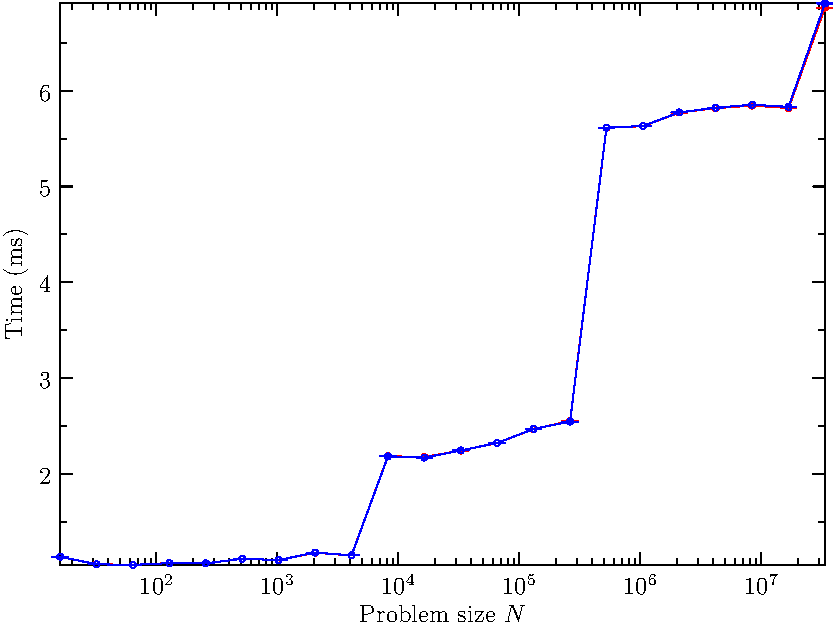
\includegraphics[width=0.5\textwidth]{pdf/meanboot.pdf}
    \end{center}
    \begin{center}
      Mean with 95\% interval from bootstrap resampling.
    \end{center}
\end{frame}
    
\begin{frame}
    \frametitle{Uncertainty quantification}
    % ./rocfft-perf --verbose  pdf ~/sync/amd/ntrial/ixt-hq-107/seq/foot/8192/doc ~/sync/amd/ntrial/ixt-hq-107/seq/foot/8192/a ~/sync/amd/ntrial/ixt-hq-107/seq/foot/8192/aa --measure median --confidence bootstrap --significance 2

    %asy -f pdf /home/mal/repo/rocfft/scripts/perf/datagraphs.asy -u 'filenames="/home/mal/sync/amd/ntrial/ixt-hq-107/seq/foot/8192/a/footprint2exp25_1D_double_backward_complex_out-of-place.mdat,/home/mal/sync/amd/ntrial/ixt-hq-107/seq/foot/8192/aa/footprint2exp25_1D_double_backward_complex_out-of-place.mdat";dobars=true;dolegend=false'  -o medianboot.pdf
    
    \begin{center}
      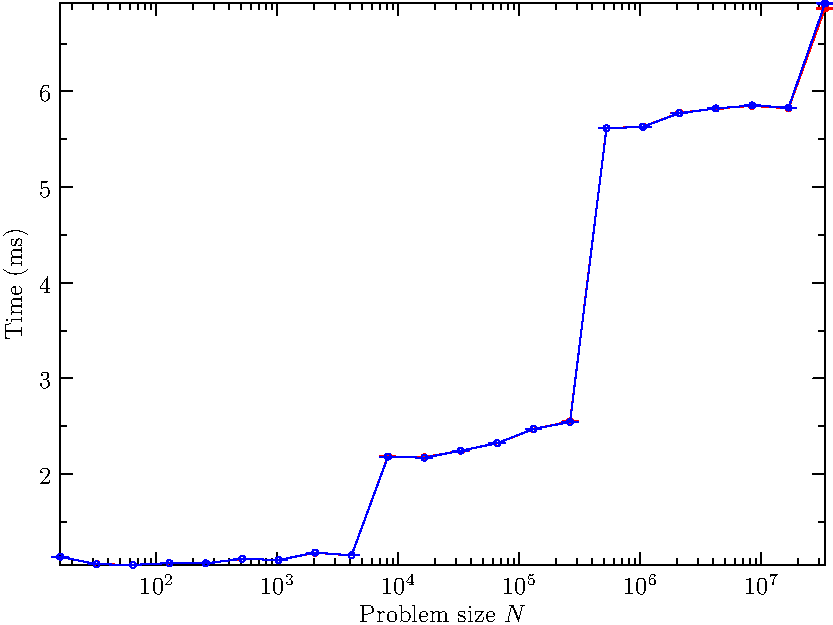
\includegraphics[width=0.5\textwidth]{pdf/medianboot.pdf}
    \end{center}
    \begin{center}
      Median with 95\% interval from bootstrap resampling.
    \end{center}
\end{frame}


\begin{frame}
  \frametitle{Uncertainty quantification: speedup}

  We're also interested in quantifying uncertainty for the speedup.

  FIXME: Describe how do we do this.
  
  %./rocfft-perf post ~/sync/amd/ntrial/ixt-hq-107/seq/foot/8192/doc ~/sync/amd/ntrial/ixt-hq-107/seq/foot/8192/a ~/sync/amd/ntrial/ixt-hq-107/seq/foot/8192/aa --measure median --confidence bootstrap

  %asy -f pdf /home/mal/repo/rocfft/scripts/perf/datagraphs.asy -u 'filenames="/home/mal/sync/amd/ntrial/ixt-hq-107/seq/foot/8192/a/footprint2exp25_1D_double_backward_complex_out-of-place.mdat,/home/mal/sync/amd/ntrial/ixt-hq-107/seq/foot/8192/aa/footprint2exp25_1D_double_backward_complex_out-of-place.mdat";legendlist="a,aa";secondary_filenames="/home/mal/sync/amd/ntrial/ixt-hq-107/seq/foot/8192/doc/aa-over-a-footprint2exp25_1D_double_backward_complex_out-of-place.sdat";dolegend=false' -o speedup.pdf

    \begin{center}
      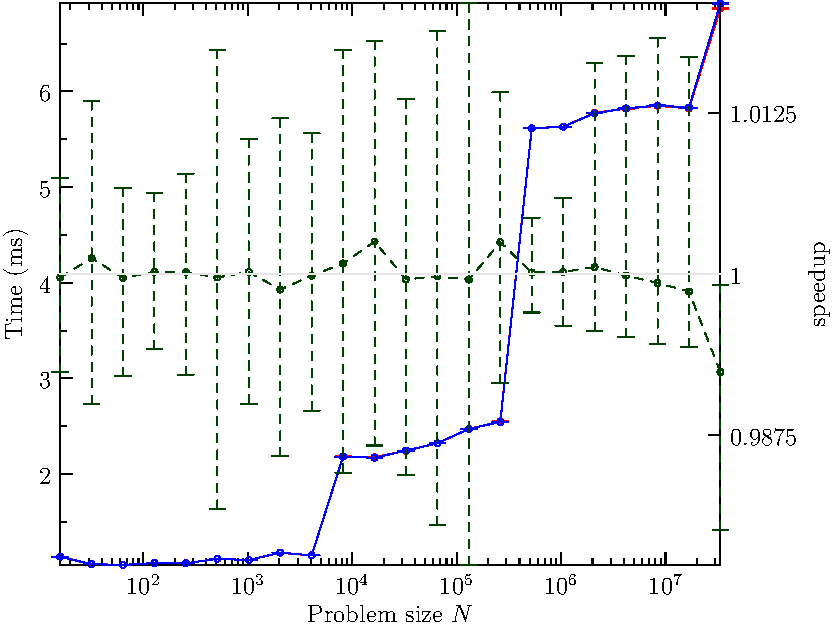
\includegraphics[width=0.5\textwidth]{pdf/speedup.pdf}
    \end{center}
    \begin{center}
      Speedup with 95\% interval from bootstrap resampling.
    \end{center}
  
\end{frame}

\begin{frame}
    \frametitle{Dealing with uncertainty}
   
    Motivation: noise in statistical tests.

    TODO: talk about how now we have iid data, we can apply tests.
    Let's also look at the data.
    
    Show: histogram of times.

    Show: histogram of speedups.
    
\end{frame}


\begin{frame}
    \frametitle{Statistical tests}


    Ref: FFTW talking about jitter.

    Ref: collective operations which handle jitter (eg alltoall - what
    if one process is slow?)
    
    Ref: Lelbach (no null-hypothesis testing), gperf (std dev)

    Show: single test.
    
    Show: as we increase bins in histogram, things get discrete.
    
    
\end{frame}


\begin{frame}
    \frametitle{Multiple hypothesis testing}

    discuss p-hacking

    Bonferroni correction

    Empirical distribution testing
    
    
\end{frame}


\begin{frame}
    \frametitle{Multiple hypothesis testing}

    Moods vs MWU vs ttest

    FIXME: Refer: that paper that talks about additive-only noise.

\end{frame}


\begin{frame}
    \frametitle{Noise vs hardware}

    Different AMD GPUs

    lockhart vs Crusher

    setting the clocks vs no

    AMD vs NVIDIA
    
\end{frame}


\begin{frame}
    \frametitle{Roberts and Son Colocation Services}

    A far better solution than what we have now.
    
\end{frame}


\begin{frame}
    \frametitle{Recommendations for Performance testing}

    Randomization

    Minimal orthogonal set of tests (best of luck eh)

    Randomize, get enough samples, use Bonferroni.

    Pick your hardware.
    
\end{frame}

\begin{frame}
    \frametitle{Use all the data}

    Longtidudinal data: how can we use this?

\end{frame}


\begin{frame}
    \frametitle{Baesean Model for Performance Tuning}

    Make use of prior knowledge and uncertainty.

\end{frame}

\end{document}
